\documentclass{beamer}
\usepackage{../../typesetting/styles/slide-zh}

% Document information
\title{\LARGE{周报}}
\subtitle{}
\author{}
\date{\today}

\begin{document}

% Title frame
\begin{frame}
  \titlepage
\end{frame}

% Outline frame
\begin{frame}{大纲}
  \tableofcontents
\end{frame}

% Paper Experiment
\section{论文实验}
\begin{frame}{自适应线程分配实验}
  \begin{block}{实验结果}
    相比\cite{Wang2025}的基准实现,我们的优化方案:
    \begin{itemize}
      \item 签名生成阶段: 性能提升\textcolor{blue}{20\%}
      \item 在资源密集型操作(如哈希计算)中效果尤为明显
    \end{itemize}
  \end{block}

  \begin{center}
    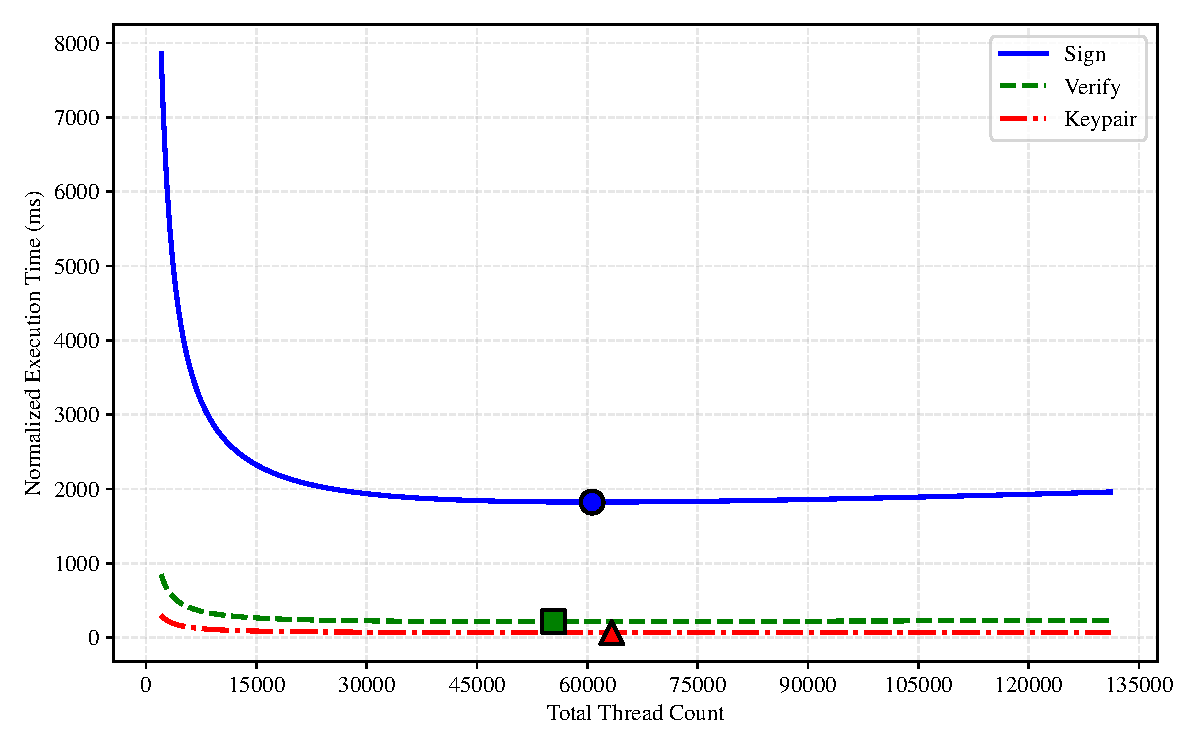
\includegraphics[width=0.7\textwidth]{./fig/thread_efficiency.pdf}
  \end{center}
\end{frame}

% Paper Writing
\section{论文写作}
\begin{frame}{口语化表达修正}
  \begin{block}{语言调整}
    我们对论文进行了全面的语言风格优化,主要包括:将一般性描述替换为更精确的专业术语,优化句法结构以消除冗余表达,重构段落组织以确保逻辑连贯,采用学术写作规范的被动语态,以及精炼图表说明文字。
  \end{block}

  \begin{center}
    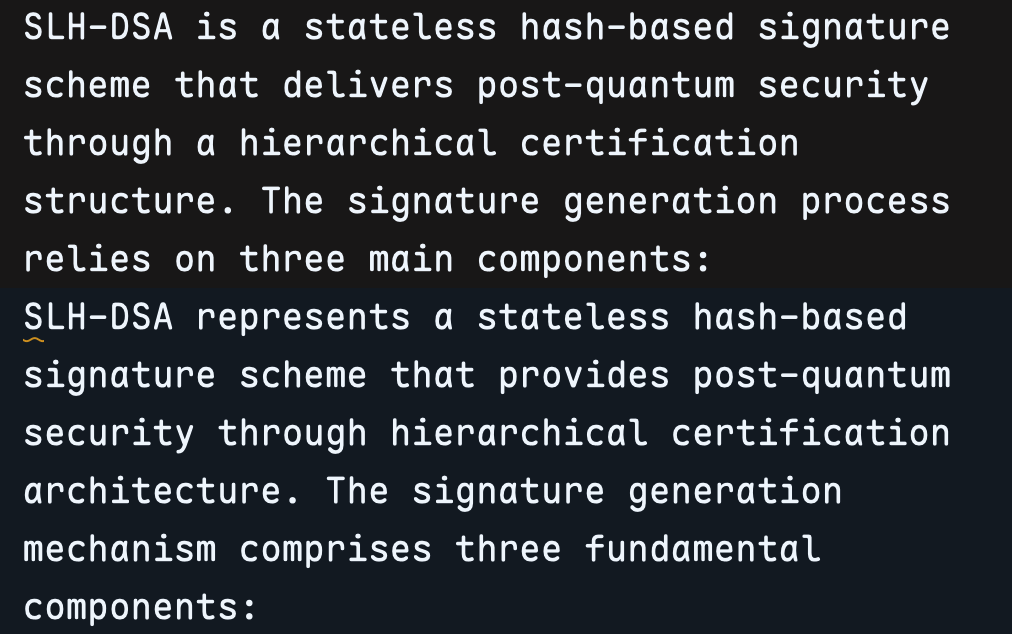
\includegraphics[width=0.65\textwidth]{./fig/fix_writing.png}
  \end{center}
\end{frame}

\begin{frame}{实验章节框架设计}
  \begin{seqpara}
    \seqsent{基于NVIDIA RTX 4090 GPU的硬件平台配置与NIST标准参数集的实验环境设置。}
    \seqsent{通过精确测量各组件执行时间定量评估ATA算法对密码学核心函数的优化贡献。}
    \seqsent{与传统串行实现对比评估FLP技术在不同安全级别下的加速效果。}
    \seqsent{与NIST参考代码和最新GPU实现进行多维度对比。}
    \seqsent{在不同安全参数下测试性能变化趋势。}
  \end{seqpara}
\end{frame}

\begin{frame}{POPE评估指标}
  \begin{block}{基本操作并行效率 (Primitive Operation Parallel Efficiency)}
    \begin{enumerate}
      \item 专门度量密码学算法基本操作P上的线程利用率
      \item 直接反映并行架构中最小计算单元的利用效率
      \item 建立密码学算法特性与并行资源分配策略的直接联系
      \item 预测不同安全参数下算法性能的可扩展性
    \end{enumerate}
  \end{block}
\end{frame}

\begin{frame}{老师评语}

  \begin{alertblock}{你觉得你现在写这篇论文遇到的最大困难是什么?}
    如何在签名组件实现,\textcolor{blue}{并行化}不能在提升的情况下,去提升性能?
  \end{alertblock}
  \vfill

  \begin{block}{下周计划}
    \begin{itemize}
      \item 完成POPE指标实验验证
      \item 准备完整的实验数据与可视化图表
    \end{itemize}
  \end{block}

\end{frame}

% References
\begin{frame}
  \frametitle{参考文献}
  \bibliographystyle{alpha}
  \bibliography{../../paper}
\end{frame}

% Thank you slide

\end{document}
